\subsection{Model Validation}
\label{subsec:model_validation}

Achieving a good in-sample fit does not necessarily guarantee that our model will also
be able to make out of sample predictions. For example, it could be that the results
are very sensitive to the exact number of vaccinations, the work mobility multiplier
or the number of rapid tests that are performed -- all of which are things that cannot
be exactly known ex-ante.

In this section we compare simulated infections that use all available data with
out of sample predictions that only use data that was available at March 1 2021.

For the out of sample predictions we predict the number of vaccinations between March
and June with a simple linear regression model that was fitted on vaccine data from
February. The work mobility multiplier is predicted to be constant at a value of
0.75, which is an approximate average of the second half of February.

The area that is frought with the most uncerainty are the introduction of rapid test,
because it comprises both, supply and demand factors. Moreover, accurately predicting
the number of rapid tests ist expected to be important because rapid tests play a large
role for the transmission dynamic.



\begin{figure}[ht] % Robustness Check
  \centering
  \begin{subfigure}[b]{.49\textwidth}
    \centering
    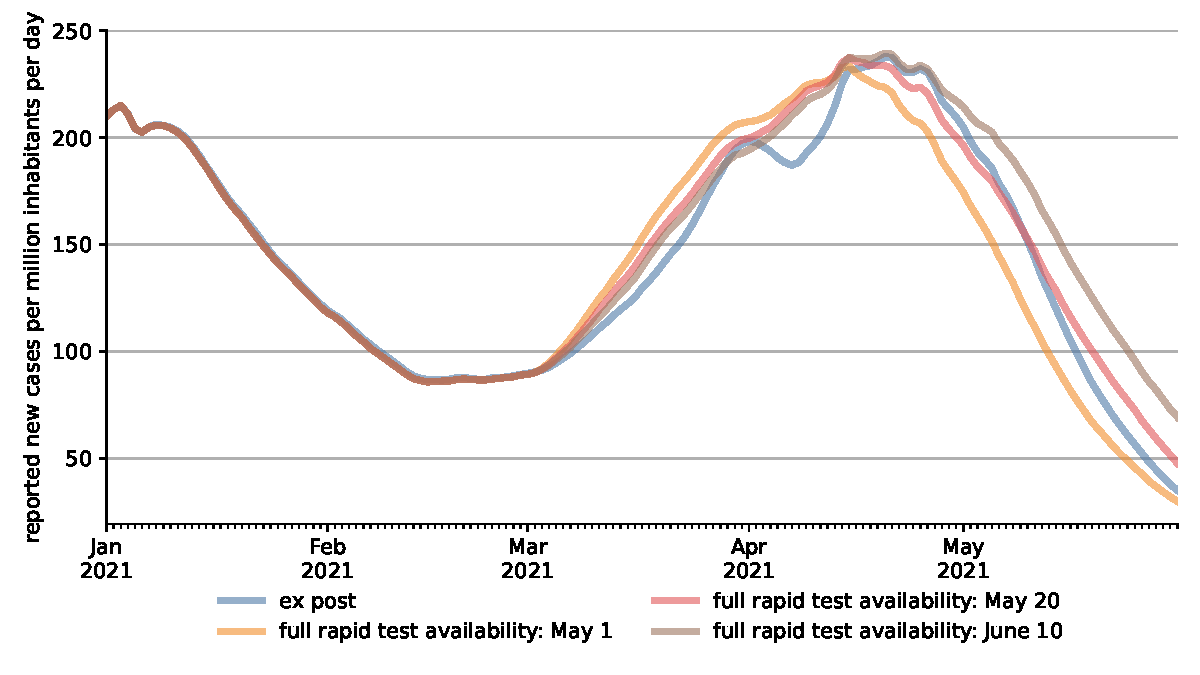
\includegraphics[width=0.9 \textwidth]{figures/results/figures/scenario_comparisons/robustness_check/full_new_known_case}
    \caption{Reported Cases}
    \label{fig:robustness_check_new_known_case}
  \end{subfigure}%
  \hfill
  \begin{subfigure}[b]{.49\textwidth}
    \centering
    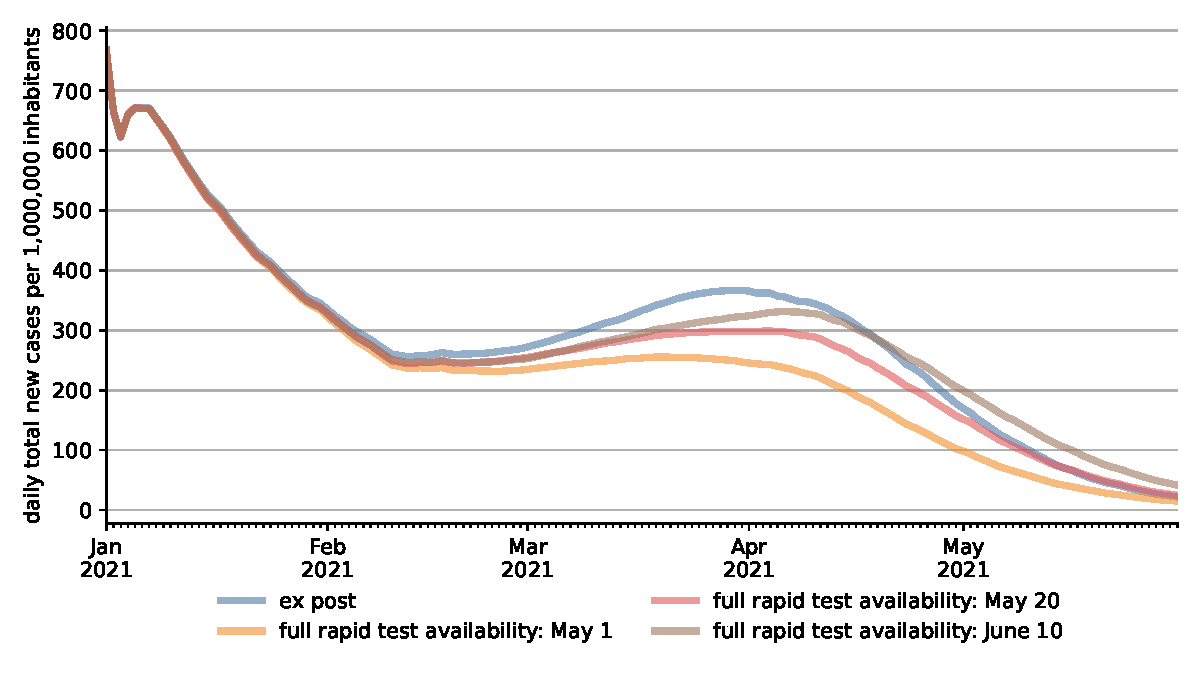
\includegraphics[width=0.9 \textwidth]{figures/results/figures/scenario_comparisons/robustness_check/full_newly_infected}
    \caption{Total Cases}
    \label{fig:robustness_check_newly_infected}
  \end{subfigure}
  \caption{Out of sample prediction for reported and total cases from March to June
    2021. The ex-post scenario is an in-sample prediction that uses all available
    information and is very close to actual case numbers. For the other scenarios data
    on vaccinations, work mobility and rapid tests that became available after March 1
    have been replaced by prediction models that are calibrated with data from February.
    Moreover, they do not model a lower number of detected cases over the easter
    holidays. The different scenarios make different assumptions on the date at which
    full availability of rapid tests is reached. While the out of sample predictions
    differ substantially for the exact case numbers at the beginning of June (between
    20 and 70 cases per million), they can all reproduce the decline in case numbers
    that is jointly driven by seasonality, large scale rapid tests and vaccinations.
  }
  \label{fig:robustness_check_detailed}
  \floatfoot{\noindent \textit{Note:} \textcolor{red}{To be written}}
\end{figure}

 \comment[id=K]{@Janos: Please add caption and description for the robustness check.}
